\documentclass[12pt,a4paper]{article}

% ─── Page Layout ───────────────────────────────────────────────────────────────
\usepackage[a4paper, margin=0.8in, headheight=14pt]{geometry}

% ─── Fonts (XeLaTeX) ───────────────────────────────────────────────────────────
\usepackage{fontspec}
\usepackage{unicode-math}
\setmainfont{TeX Gyre Pagella}
\setmonofont[Scale=0.88]{TeX Gyre Cursor}
\setmathfont{Latin Modern Math}

% ─── Packages ──────────────────────────────────────────────────────────────────
\usepackage{xcolor}
\usepackage{colortbl}
\usepackage{titlesec}
\usepackage{enumitem}
\usepackage{tabularx}
\usepackage{booktabs}
\usepackage{array}
\usepackage{amsmath}
\usepackage{tikz}
\usetikzlibrary{shapes.geometric, arrows.meta, positioning, calc, fit, decorations.pathreplacing}
\usepackage{tcolorbox}
\tcbuselibrary{skins, breakable}
\usepackage{hyperref}
\usepackage{fancyhdr}
\usepackage{graphicx}
\usepackage{microtype}
\hyphenpenalty=10000
\exhyphenpenalty=10000
\sloppy
\usepackage{caption}
\usepackage{setspace}
\usepackage{multirow}
\usepackage{tocloft}

% ─── Q&A helper ────────────────────────────────────────────────────────────────
\newcommand{\Q}[1]{\textbf{#1}\par\noindent\ignorespaces}

% ─── Colour Palette ────────────────────────────────────────────────────────────
\definecolor{myred}{RGB}{196,30,58}
\definecolor{mydark}{RGB}{30,30,50}
\definecolor{mygreen}{RGB}{14,120,80}
\definecolor{myteal}{RGB}{0,130,140}
\definecolor{myamber}{RGB}{180,100,0}
\definecolor{mypurple}{RGB}{100,30,160}
\definecolor{mygray}{RGB}{246,247,249}
\definecolor{mgframe}{RGB}{180,185,200}
\definecolor{watermark}{RGB}{145,150,170}
\definecolor{hdrred}{RGB}{250,232,235}
\definecolor{hdrgreen}{RGB}{220,244,233}
\definecolor{hdrteal}{RGB}{220,242,244}
\definecolor{hdramber}{RGB}{253,242,215}
\definecolor{hdrpurple}{RGB}{238,228,255}
\definecolor{hdrgray}{RGB}{238,240,245}
\definecolor{rowalt}{RGB}{250,251,253}

% ─── Section Formatting ────────────────────────────────────────────────────────
\titleformat{\section}
  {\large\bfseries\color{myred}}{\thesection.}{0.5em}{}
  [\vspace{1pt}{\color{myred}\rule{\linewidth}{0.8pt}}]
\titleformat{\subsection}
  {\normalsize\bfseries\color{myteal}}{\thesubsection}{0.5em}{}
\titlespacing*{\section}{0pt}{18pt}{7pt}
\titlespacing*{\subsection}{0pt}{11pt}{4pt}

% ─── Paragraph ─────────────────────────────────────────────────────────────────
\setlength{\parindent}{0pt}
\setlength{\parskip}{4pt}

% ─── TOC Styling ───────────────────────────────────────────────────────────────
\renewcommand{\cfttoctitlefont}{\large\bfseries\color{myred}}
\renewcommand{\cftaftertoctitle}{\par\noindent{\color{myred}\rule{\linewidth}{0.8pt}}}
\setlength{\cftbeforetoctitleskip}{0pt}
\setlength{\cftaftertoctitleskip}{6pt}
\renewcommand{\cftsecfont}{\normalsize\bfseries\color{mydark}}
\renewcommand{\cftsecpagefont}{\normalsize\bfseries\color{mydark}}
\renewcommand{\cftsecleader}{\cftdotfill{\cftdotsep}}
\setlength{\cftbeforesecskip}{7pt}
\renewcommand{\cftsubsecfont}{\small\color{mydark}}
\renewcommand{\cftsubsecpagefont}{\small\color{mydark}}
\setlength{\cftbeforesubsecskip}{3pt}
\setlength{\cftsubsecindent}{1.4em}

% ─── Table helpers ─────────────────────────────────────────────────────────────
\renewcommand{\arraystretch}{1.45}
\setlength{\tabcolsep}{6pt}
\arrayrulecolor{mydark}
\newcolumntype{B}[1]{>{\small\bfseries\raggedright\arraybackslash}m{#1}}
\newcolumntype{Y}{>{\small\raggedright\arraybackslash}X}
\renewcommand{\tabularxcolumn}[1]{m{#1}}

% ─── Header / Footer ───────────────────────────────────────────────────────────
\pagestyle{fancy}
\fancyhf{}
\fancyhead[L]{\small\color{myred}\textbf{OE-EC604B}\;\color{mydark}--- Operating System}
\fancyhead[R]{\small\color{myteal}\textbf{Module 7 Notes}}
\fancyfoot[C]{\small\color{mydark}\thepage}
\fancyfoot[R]{\small\color{watermark}\textit{\copyright\ Biraj}}
\renewcommand{\headrulewidth}{0.5pt}
\renewcommand{\footrulewidth}{0.3pt}

% ─── Hyperref ──────────────────────────────────────────────────────────────────
\hypersetup{
  colorlinks=true, linkcolor=myteal, urlcolor=myteal,
  pdfauthor={Biraj Sarkar},
  pdftitle={OE-EC604B --- Module 7 Notes}
}

% ─── tcolorbox styles ──────────────────────────────────────────────────────────
\tcbset{
  tikzbox/.style={
    colback=mygray, colframe=mgframe, boxrule=0.6pt, arc=4pt,
    left=8pt, right=8pt, top=6pt, bottom=6pt,
    colbacktitle=mgframe, coltitle=mydark,
    fonttitle=\small\bfseries
  },
  defbox/.style={
    colback=hdrgreen, colframe=mygreen, boxrule=0.8pt, arc=4pt,
    left=9pt, right=9pt, top=6pt, bottom=6pt,
    colbacktitle=mygreen, coltitle=white,
    fonttitle=\small\bfseries
  },
  formulabox/.style={
    colback=hdrteal, colframe=myteal, boxrule=0.8pt, arc=4pt,
    left=9pt, right=9pt, top=7pt, bottom=7pt,
    colbacktitle=myteal, coltitle=white,
    fonttitle=\small\bfseries
  },
  examplebox/.style={
    colback=hdramber, colframe=myamber, boxrule=0.8pt, arc=4pt,
    left=9pt, right=9pt, top=6pt, bottom=6pt,
    colbacktitle=myamber, coltitle=white,
    fonttitle=\small\bfseries
  },
  masonbox/.style={
    colback=hdrpurple, colframe=mypurple, boxrule=0.8pt, arc=4pt,
    left=9pt, right=9pt, top=6pt, bottom=6pt,
    colbacktitle=mypurple, coltitle=white,
    fonttitle=\small\bfseries
  },
  exambox/.style={
    colback=hdrpurple, colframe=mypurple, boxrule=1pt, arc=5pt,
    left=10pt, right=10pt, top=8pt, bottom=8pt,
    colbacktitle=mypurple, coltitle=white,
    fonttitle=\bfseries,
    breakable, title after break={\textbf{Frequently Asked / Viva Questions (contd.)}}}
}
% Make all boxes breakable across pages
\tcbset{breakable}

% ─── TikZ styles ───────────────────────────────────────────────────────────────
\tikzset{
  block/.style={rectangle, draw=myteal, fill=hdrteal,
    text width=2.4cm, align=center, minimum height=0.95cm,
    font=\small, rounded corners=3pt, line width=0.7pt},
  redblock/.style={rectangle, draw=myred, fill=hdrred,
    text width=2.4cm, align=center, minimum height=0.95cm,
    font=\small, rounded corners=3pt, line width=0.7pt},
  greenblock/.style={rectangle, draw=mygreen, fill=hdrgreen,
    text width=2.4cm, align=center, minimum height=0.95cm,
    font=\small, rounded corners=3pt, line width=0.7pt},
  amberblock/.style={rectangle, draw=myamber, fill=hdramber,
    text width=2.4cm, align=center, minimum height=0.95cm,
    font=\small, rounded corners=3pt, line width=0.7pt},
  purpblock/.style={rectangle, draw=mypurple, fill=hdrpurple,
    text width=2.4cm, align=center, minimum height=0.95cm,
    font=\small, rounded corners=3pt, line width=0.7pt},
  sumjunc/.style={circle, draw=myamber, fill=hdramber,
    minimum size=0.62cm, font=\small, line width=0.8pt},
  arrow/.style={-Stealth, thick, color=mydark},
  redarrow/.style={-Stealth, thick, color=myred},
  line/.style={thick, color=mydark}
}

% ═══════════════════════════════════════════════════════════════════════════════
\begin{document}
% ═══════════════════════════════════════════════════════════════════════════════

\begin{center}
  {\LARGE\bfseries\color{myred} OE-EC604B --- Operating System}\\[5pt]
  {\normalsize\color{mydark} Semester VI \quad$\bullet$\quad 3L:0T:0P \quad$\bullet$\quad 3 Credits}\\[3pt]
  {\normalsize\color{myteal}\textbf{Module 7 Exam Notes: I/O Management and Disk Scheduling}}\\[3pt]
  {\small\color{mydark} CGEC \;$|$\; B.Tech ECE (2023--27) \;$|$\; \textit{Biraj Sarkar}}
\end{center}
\vspace{2pt}
\noindent{\color{myred}\rule{\linewidth}{1.5pt}}
\vspace{2pt}

\hypersetup{linkcolor=mydark}
\tableofcontents
\hypersetup{linkcolor=myteal}
\newpage

% ===============================================================================
\section{I/O Hardware and Organization of I/O Functions}
% ===============================================================================

The control of I/O devices connected to the computer is a major function of an operating system. The OS must issue commands to devices, catch interrupts, and handle errors.

\subsection{I/O Communication Methods}
\begin{itemize}[leftmargin=*, itemsep=3pt]
  \item \textbf{Polling (Busy-Wait I/O):} CPU repeatedly reads the status register of the device controller until the device is ready. *Drawback:* Wastes CPU cycles.
  \item \textbf{Interrupt-Driven I/O:} CPU starts I/O and switches to other tasks. When I/O is ready, the device controller triggers a hardware interrupt, forcing the CPU to branch to the Interrupt Service Routine (ISR).
  \item \textbf{Direct Memory Access (DMA):} Used for high-speed I/O. The DMA controller transfers blocks of data directly between device buffer and main memory, interrupting the CPU only once at the end of the block transfer.
\end{itemize}

\subsection{I/O Buffering}
A buffer is a memory area that stores data temporarily while it is being transferred between two devices or between a device and an application.
\begin{itemize}[leftmargin=*, itemsep=3pt]
  \item \textbf{Single Buffering:} OS assigns a buffer in system memory. The I/O device writes to this buffer, and then the OS copies it to user space.
  \item \textbf{Double Buffering (Ping-Ponging):} OS assigns two buffers. While the user process consumes data from buffer 1, the device writes to buffer 2 in parallel.
  \item \textbf{Circular Buffering:} A queue of three or more buffers used when bursty transfer rates fluctuate.
\end{itemize}

\begin{tcolorbox}[tikzbox, title={Double Buffering Model}]
\centering
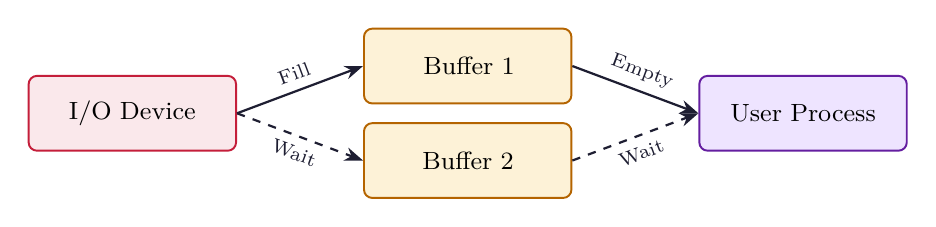
\begin{tikzpicture}[node distance=1.1cm and 1.6cm, thick, font=\small]
  \node[block, fill=hdrred, draw=myred] (dev) {I/O Device};
  \node[block, right=1.6cm of dev, fill=hdramber, draw=myamber, yshift=0.6cm] (buf1) {Buffer 1};
  \node[block, right=1.6cm of dev, fill=hdramber, draw=myamber, yshift=-0.6cm] (buf2) {Buffer 2};
  \node[block, right=1.6cm of buf1, fill=hdrpurple, draw=mypurple, yshift=-0.6cm] (user) {User Process};

  \draw[arrow] (dev.east) -- node[above, font=\scriptsize, sloped] {Fill} (buf1.west);
  \draw[arrow, dashed] (dev.east) -- node[below, font=\scriptsize, sloped] {Wait} (buf2.west);
  \draw[arrow] (buf1.east) -- node[above, font=\scriptsize, sloped] {Empty} (user.west);
  \draw[arrow, dashed] (buf2.east) -- node[below, font=\scriptsize, sloped] {Wait} (user.west);
\end{tikzpicture}
\end{tcolorbox}

% ===============================================================================
\section{Disk Physical Structure and Access Performance}
% ===============================================================================

Magnetic disks provide the bulk of secondary storage for modern systems.
\begin{itemize}[leftmargin=*, itemsep=3pt]
  \item \textbf{Structure:} Disks consist of platters coated with magnetic material. Each platter surface is divided into concentric circles called \textbf{tracks}, which are split into small sectors (typically $512\,\text{Bytes}$). Corresponding tracks on all platters form a \textbf{cylinder}.
  \item \textbf{Disk Access Time:}
  \begin{itemize}[leftmargin=*, itemsep=2.5pt, topsep=0pt]
    \item \textbf{Seek Time ($T_s$):} Time required to move the disk arm to the target cylinder. (Dominates disk latency).
    \item \textbf{Rotational Latency ($T_r$):} Time for the target sector to rotate under the read-write head. (Avg latency = $\frac{1}{2} \times$ time for one rotation).
    \item \textbf{Transfer Time ($T_t$):} Time to actually read/write data. $T_t = \frac{b}{r \cdot N}$ where $b$ = bytes to transfer, $r$ = rotation speed, $N$ = bytes per track.
    \end{itemize}
  \end{itemize}

% ===============================================================================
\section{Disk Scheduling Algorithms}
% ===============================================================================

Because seek time dominates access latency, the OS schedules incoming disk requests to minimize head travel distance.

\subsection*{Request Queue Example}
For the algorithms below, assume a disk with 200 cylinders (0–199). The request queue is:
\texttt{98, 183, 37, 122, 14, 124, 65, 67}. Read-write head starts at cylinder \textbf{53}.

\subsection{First-Come, First-Served (FCFS)}
\begin{itemize}[leftmargin=*, itemsep=3pt]
  \item \textbf{Working:} Services requests in the order of arrival.
  \item \textbf{Head Movement Path:} $53 \to 98 \to 183 \to 37 \to 122 \to 14 \to 124 \to 65 \to 67$.
  \item \textbf{Total head cylinders traversed:} 640. Fair, but very inefficient.
\end{itemize}

\subsection{Shortest Seek Time First (SSTF)}
\begin{itemize}[leftmargin=*, itemsep=3pt]
  \item \textbf{Working:} Selects the request closest to the current head position.
  \item \textbf{Head Movement Path:} $53 \to 65 \to 67 \to 37 \to 14 \to 98 \to 122 \to 124 \to 183$.
  \item \textbf{Total head cylinders traversed:} 236. High efficiency but prone to \textbf{starvation} of outer cylinders.
\end{itemize}

\subsection{SCAN (Elevator Algorithm)}
\begin{itemize}[leftmargin=*, itemsep=3pt]
  \item \textbf{Working:} Arm starts at one end, moves toward the other end, servicing requests, until it reaches the boundary (cylinder 0 or 199), then reverses direction.
  \item \textbf{Head Movement Path (moving towards 0):} $53 \to 37 \to 14 \to \mathbf{0} \to 65 \to 67 \to 98 \to 122 \to 124 \to 183$.
  \item \textbf{Total head cylinders traversed:} 236. Prevents starvation, but treats boundary requests unfairly.
\end{itemize}

\subsection{C-SCAN (Circular SCAN)}
\begin{itemize}[leftmargin=*, itemsep=3pt]
  \item \textbf{Working:} Moves from one end to the other servicing requests. When it reaches the end, it immediately returns to the starting boundary without servicing any requests on the return trip.
  \item \textbf{Head Movement Path (moving towards 199):} $53 \to 65 \to 67 \to 98 \to 122 \to 124 \to 183 \to \mathbf{199} \to \mathbf{0} \to 14 \to 37$.
  \item \textbf{Total head cylinders traversed:} 382. Provides more uniform waiting times.
\end{itemize}

\subsection{LOOK \& C-LOOK}
\begin{itemize}[leftmargin=*, itemsep=3pt]
  \item \textbf{Working:} Similar to SCAN and C-SCAN but the arm goes only as far as the \textbf{last request} in each direction, rather than traveling to the extreme boundaries (0 or 199).
  \item \textbf{C-LOOK Path (moving towards 183):} $53 \to 65 \to 67 \to 98 \to 122 \to 124 \to 183 \to \mathbf{14} \to 37$.
  \item \textbf{Total head cylinders traversed:} 322. Saves travel time compared to C-SCAN.
\end{itemize}

\newpage
% ===============================================================================
% MANDATORY QUICK REVISION PAGE
% ===============================================================================
\begin{center}
  {\large\bfseries\color{myred} Quick Revision --- Module 7}\\[3pt]
  {\small\color{mydark} I/O Management and Disk Scheduling $|$ OE-EC604B}
\end{center}
\noindent{\color{myred}\rule{\linewidth}{1.2pt}}
\vspace{4pt}

\begin{tcolorbox}[formulabox, title={\textbf{Disk Parameter Definitions}}]
$$\text{Total Disk Access Time} = \text{Seek Time} + \text{Rotational Latency} + \text{Transfer Time}$$
$$\text{Average Rotational Latency} = \frac{1}{2} \times \frac{60}{\text{RPM}}\ \text{seconds}$$
\end{tcolorbox}

\begin{tcolorbox}[defbox, title={\textbf{One-Line Definitions}}]
\begin{itemize}[leftmargin=*, itemsep=2.5pt, topsep=0pt]
  \item \textbf{DMA:} Direct Memory Access; I/O technique transferring data blocks to memory without CPU overhead.
  \item \textbf{Double Buffering:} OS buffering model using two registers in parallel to remove consumption stalls.
  \item \textbf{Seek Time:} Time taken for the read-write head assembly to align with the target cylinder.
  \item \textbf{Rotational Latency:} Time taken for the target sector to rotate under the active head.
  \item \textbf{SSTF:} Shortest Seek Time First; scheduling that selects request with minimal seek distance.
  \item \textbf{SCAN:} Elevator scheduling algorithm traversing the entire disk width in cycles.
  \item \textbf{C-SCAN:} Circular SCAN; sweeps in one direction, returning to start instantly without serving.
  \item \textbf{C-LOOK:} SCAN variant that returns immediately after servicing the last request in that direction.
\end{itemize}
\end{tcolorbox}

\begin{tcolorbox}[exambox, title={\textbf{Frequently Asked / Viva Questions}}]
\begin{enumerate}[topsep=0pt, label=\textbf{Q\arabic*.}, itemsep=5pt]
  \item \Q{Explain the difference between Polling, Interrupt-driven I/O, and DMA.}
    Polling has the CPU busy-wait checking status registers. Interrupt-driven I/O triggers hardware interrupts when data is ready, letting the CPU execute other tasks. DMA uses a dedicated controller to transfer large blocks directly between device and memory, interrupting the CPU only once at block completion.
  \item \Q{Compare SCAN, C-SCAN, LOOK, and C-LOOK disk scheduling algorithms.}
    SCAN moves the head to the extreme boundary in one direction, then reverses. C-SCAN goes to the boundary, returns to the other boundary without servicing on the return. LOOK and C-LOOK improve on this by reversing at the last request instead of going to the extreme boundary.
  \item \Q{Give a numerical comparison of SCAN vs LOOK head travel. Head starts at 50 (direction: increasing). Request queue: \texttt{90, 150, 20}. Boundary = 199.}
    *SCAN:* Head goes $50 \to 90 \to 150 \to \mathbf{199} \to 20$. Head travel: $(199 - 50) + (199 - 20) = 149 + 179 = 328$ cylinders.\par
    *LOOK:* Head goes $50 \to 90 \to 150 \to 20$ (stops at 150 because it is the last request). Head travel: $(150 - 50) + (150 - 20) = 100 + 130 = 230$ cylinders.
  \item \Q{What is starvation in disk scheduling? Which algorithm is most prone to it?}
    Starvation occurs when a request is never serviced because closer requests keep arriving. SSTF is most prone to starvation because the head tends to stay in localized clusters, leaving requests on the far ends unserviced.
  \item \Q{Explain the mechanical layout of a Hard Disk Drive.}
    A spindle holds multiple circular platters. Read-write heads are mounted on an actuator arm that moves radially. Each platter surface contains concentric tracks, and tracks are divided into sectors. Corresponding tracks vertically form cylinders.
  \item \Q{What is double buffering and why is it preferred over single buffering?}
    Double buffering assigns two buffers. While the CPU reads/empties buffer 1, the device controller fills buffer 2 concurrently. In single buffering, the CPU must stall while the single buffer is being re-filled.
  \item \Q{Define Seek Time, Rotational Latency, and Transfer Time.}
    Seek time is the time to align the arm over the cylinder. Rotational latency is the time for the sector to rotate to the head. Transfer time is the actual data read/write rate.
  \item \Q{A disk rotates at 7200 RPM. What is its average rotational latency?}
    7200 rotations in 60 seconds $\to 1$ rotation takes $60 / 7200 = 8.33\,\text{ms}$. Average rotational latency is half of one rotation time: $0.5 \times 8.33 = 4.17\,\text{ms}$.
  \item \Q{Why does C-SCAN offer more uniform waiting times than SCAN?}
    In SCAN, cylinders near the middle are swept twice as often as those near the boundaries. C-SCAN sweeps in one direction only, returning to start instantly, giving all cylinders a uniform wait interval between sweeps.
  \item \Q{What are the main design issues in I/O system design?}
    Achieving device independence (programs can write to any device without custom code), uniform naming, error handling, buffering optimization, and asynchronous operation.
\end{enumerate}
\end{tcolorbox}

\begin{tcolorbox}[tikzbox, title={Disk Scheduling Algorithms Comparison}]
\renewcommand{\arraystretch}{1.4}
\par\noindent
\begin{tabularx}{\linewidth}{|B{2.2cm}|>{\small\centering\arraybackslash}X|>{\small\centering\arraybackslash}X|>{\small\centering\arraybackslash}X|}
\hline
\textbf{Algorithm} & \textbf{\color{myred}Average Seek Time} & \textbf{\color{myteal}Starvation Risk?} & \textbf{\color{myamber}Boundary Travel?} \\
\hline
\textbf{FCFS} & High (non-optimal) & No & No \\
\hline
\textbf{SSTF} & Low (highly localized) & Yes & No \\
\hline
\textbf{SCAN} & Low & No & Yes (goes to end) \\
\hline
\textbf{C-LOOK} & Low to Moderate & No & No (reverses at last request) \\
\hline
\end{tabularx}
\end{tcolorbox}

\end{document}
